\section{Evaluation}
% To develop a preliminary understanding of the energy contributions of the model reconfiguration from external memory, we evaluate a variety of realistic and applicable models.
% The power is the configuration of a model and a single inference with the model at \SI{60}{FPS}.
% Effectively, this means that the same model is configured on the \graicore{} 60 times per second and also used to proces an input frame 30 times per second.

To develop a preliminary understanding of the energy contributions of the model reconfiguration from external memory, we evaluate a variety of realistic and applicable models.
We will be looking at two different external memory technologies, LPDDR5X and PCM.
LPDDR5X is chosen for its high bandwidth and density, while PCM is selected for its potential to reduce energy consumption due to its non-volatility.
We assume we use the DDR protocol for transferring data to the AXI bus that is connected to the \graicore{}.
For the DDR protocol to work, we require an DDR PHY and DDR controller.
These components both add to the energy when transferring data to the \graicore{}.

% \begin{table}[hbtp]
%     \centering
%     \begin{threeparttable}
%         \begin{tabular}{@{}lrl@{}}
%         \toprule
%         \textbf{Component} & \textbf{Value} & \textbf{Unit} \\
%         \midrule
%         LPDDR5X read\tnote{1}               & 36.00 & pJ/B \\
%         PCM read\tnote{2}                   & 5.29  & pJ/B \\
%         DDR PHY\tnote{3}                    & 10.39 & pJ/B \\
%         DDR Controller\tnote{3}             & 1.56  & pJ/B \\
%         AXI Bus\tnote{3}                    & 6.25  & pJ/B \\
%         \confignoc{} hop (64 bits)\tnote{3} & 0.26  & pJ   \\
%         SRAM write (64 bits)\tnote{3}       & 4.98  & pJ   \\ \bottomrule
%         \end{tabular}
%         \begin{tablenotes}
%             \item[1] From internal research of the MT62F1G16D1 memory chip from Micron.
%             \item[2] From internal research of a custom PCM memory architecture.
%             \item[3] From internal measurements.
%             % \item[3] From internal measurements (\SI{133}{mW} at full capacity).
%             % \item[4] From internal measurements (\SI{20}{mW} at full capacity).
%             % \item[5] From internal measurements (\SI{80}{mW} at full capacity).
%         \end{tablenotes}
%     \end{threeparttable}
%     \caption{Energy parameters of PCM and LPDDR5X memory, DDR interface and \graicore{} that are relevant for model configuration}
%     \label{tab:energy_parameters}
% \end{table}

We look at the models as shown in \cref{tab:example_models_stats}.
It also shows the processing latency, the number of cores used and the average utilization of the cores of each (mapped) model.
These statistics are used for computing the processing energy.
The ``to write'' column shows the total amount of bytes that is to be transferred to the \graicore{} for the corresponding model.
Note that to get a more accurate energy number for configuration, we need the amount of bytes to be transferred to each core individually.
This information is available, and will be used for the evaluation.

\begin{table}[hbtp]
\centering
\begin{tabular}{@{}lrrrrr@{}}
\toprule
\textbf{Model}          & \textbf{\begin{tabular}[c]{@{}l@{}}Latency\\ (ms)\end{tabular}} & \textbf{\begin{tabular}[c]{@{}l@{}}Cores\\used\end{tabular}} & \textbf{Avg util.} & \textbf{\begin{tabular}[c]{@{}l@{}}To write\\ (MiB)\end{tabular}} \\ \midrule
efficientnet            & 1.642                                                           & 144            & 50.89\%            & 16.15                                                             \\
mobnetv2                & 1.296                                                           & 144            & 40.78\%            & 10.67                                                             \\
object\_tracker         & 1.480                                                           & 144            & 36.62\%            & 12.33                                                             \\
object\_detector        & 4.809                                                           & 144            & 68.03\%            & 19.12                                                             \\
resnet50                & 5.765                                                           & 144            & 36.35\%            & 29.58                                                             \\
resnet101\_p0           & 7.080                                                           & 144            & 33.40\%            & 28.75                                                             \\
resnet101\_p1           & 2.647                                                           & 143            & 36.42\%            & 20.06                                                             \\
resnet101\_p2           & 4.011                                                           & 144            & 33.12\%            & 30.44                                                             \\
resnet101\_p3           & 2.343                                                           & 143            & 33.55\%            & 17.71                                                             \\
resnet101\_p4           & 2.040                                                           & 143            & 26.19\%            & 15.54                                                             \\
resnet101\_pruned\_p0   & 6.552                                                           & 144            & 38.10\%            & 15.87                                                             \\
resnet101\_pruned\_p1   & 3.245                                                           & 143            & 34.31\%            & 10.43                                                             \\
resnet101\_pruned\_p2   & 4.501                                                           & 143            & 33.83\%            & 16.00                                                             \\
resnet101\_pruned\_p3   & 2.114                                                           & 143            & 38.08\%            & 10.22                                                             \\
resnet101\_pruned\_p4   & 2.437                                                           & 143            & 24.25\%            & 7.69                                                              \\
\bottomrule
\end{tabular}
\caption{
    Statistics of various mapped models.
    The latency, cores used and average utilization are obtained from simulations with the performance simulator.
    The amount of bytes to write are obtained from the compiler artifacts.
}
\label{tab:example_models_stats}
\end{table}

% As an example, we demonstrate a calculation for the ResNet-50 model.
% The processing energy is calculated as follows (assuming an average core power of \SI{21}{mW}\footnote{This constant is obtained from internal RTL simulations.}):
% \begin{equation}
%     \eproc = 0.3635 \times 144 \times \SI{5.765}{ms} \times \SI{21}{mW} = \SI{6.34}{mJ}
% \end{equation}

\Cref{fig:model_data_heapmap} shows for the mapped ResNet-50 the amount of data to be sent to each individual core.
We use this information to construct matrix $D$ and the configuration energy $\econf$.
Finally, we compute the values as presented in \cref{fig:resnet50_conf_energy_distribution}.
% Finally, we compute the values as presented in \cref{tab:resnet50_energy}.
% Configuration with LPDDR5X of the ResNet-50 model on the \graicore{} consumes \SI{1.71}{mJ} and with PCM \SI{0.76}{mJ}.

% \begin{table}[hbtp]
%     \centering
%     \begin{tabular}{@{}lr@{}}
%     \toprule
%     \textbf{Component} & \textbf{Value} \\
%     \midrule
%     $\ereadlpddr5x$ & 1116.8 \\
%     $\ereadpcm$ & 164.2 \\
%     $\ephy$ & 322.4 \\
%     $\ectrl$ & 48.5 \\
%     $\eaxi$ & 193.9 \\
%     $\enoc$ & 9.2 \\
%     $\ewrite$ & 19.3 \\
%     \bottomrule
%     \end{tabular}
%     \caption{
%         Computed energy values for each relevant component during configuration.
%         All values shown are in \SI{}{\micro\joule}.
%     }
%     \label{tab:resnet50_energy}
% \end{table}

% Then, the total energy consumption when performing a single configuration and a single inference is \SI{8.05}{mJ} for LPDDR5X and \SI{7.09}{mJ} for PCM.

\begin{figure}[hbtp]
    \centering
    \subcaptionbox{LPDDR5X\label{fig:pie_resnet50_conf_lpddr5x}}{
        \import{assets/power_analysis}{pre}
\begin{tikzpicture}
    \pie[
        radius=2,
        text=pin,
        color = {blue!60, blue!50, blue!40, blue!30, blue!20, blue!10},
        before number=\printonlylargeenough{10},
        after number=\ifprintnumber\%\fi
    ]{
        64.9/$\eread$,
        19.3/$\ephy$,
        2.8/$\ectrl$,
        11.3/$\eaxi$,
        0.5/$\enoc$,
        1.1/$\ewrite$
    }
\end{tikzpicture}

    }
    \hfill
    \subcaptionbox{PCM\label{fig:pie_resnet50_conf_pcm}}{
        \import{assets/power_analysis}{pre}
\begin{tikzpicture}
    \pie[
        radius=1.8,
        text=pin,
        color = {blue!60, blue!50, blue!40, blue!30, blue!20, blue!10},
        before number=\printonlylargeenough{10},
        after number=\ifprintnumber\%\fi
    ]{
        % 21.4/$\eread$,
        % 43.3/$\ephy$,
        % 6.3/$\ectrl$,
        % 25.3/$\eaxi$,
        % 1.2/$\enoc$,
        % 2.5/$\ewrite$
        21.4/$\eread$,
        43.3/$\ephy$,
        % 6.3/$\ectrl$,
        25.3/$\eaxi$,
        10.0/$\textrm{other}$
        % 1.2/$\enoc$,
        % 2.5/$\ewrite$
    }
\end{tikzpicture}

    }
    \caption{ResNet-50 configuration energy distribution. The ``other'' slice includes $\ectrl$, $\enoc$ and $\ewrite$.}
    \label{fig:resnet50_conf_energy_distribution}
\end{figure}

% Looking at the configuration energy, with LPDDR5X, most of the energy is consumed by reading from the external memory (see \cref{fig:resnet50_conf_energy_distribution}).
Looking at the configuration energy, with LPDDR5X, most of the energy is consumed by reading from the external memory.
While for PCM, most of the energy is consumed by the DDR PHY.

\begin{figure}[hbtp]
    \centering
    \subcaptionbox{LPDDR5X\label{fig:pie_resnet50_conf_proc_lpddr5x}}{
        \begin{tikzpicture}
    \pie[
        radius=1.8,
        text=pin,
        color={blue!60, red!60},
    ]{
        21.2/$\econf$,
        78.8/$\eproc$
    }
\end{tikzpicture}

    }
    \hfill
    \subcaptionbox{PCM\label{fig:pie_resnet50_conf_proc_pcm}}{
        \begin{tikzpicture}
    \pie[
        radius=1.8,
        text=pin,
        color={blue!60, red!60},
    ]{
        10.7/$\econf$,
        89.3/$\eproc$
    }
\end{tikzpicture}

    }
    \caption{Configuration vs. processing energy for the ResNet-50 model}
    \label{fig:resnet50_conf_proc}
\end{figure}

Shown in \cref{fig:resnet50_conf_proc}, the configuration of the ResNet-50 model occupies around 21\% with LPDDR5X and 11\% with PCM of the total energy consumption (this includes both processing and configuration).
Of all the models listed in \cref{tab:example_models_stats}, on average, around 23\% is used for configuration with LPDDR5X memory and 12\% with PCM as external memory (see \cref{fig:example_models_avg_conf_proc}).

\begin{figure}[hbtp]
    \centering
    \subcaptionbox{LPDDR5X\label{fig:sunburst_avg_conf_proc_lpddr5x}}{
        \import{assets/power_analysis}{pre}
\begin{tikzpicture}
    \pie[
        radius=2.5,
        text=pin,
        hide number,
    ]{
        1.0/1.0\%,
        14.9/14.9\%,
        4.3/4.3\%,
        2.8/2.8\%
    }
    \pie[
        radius=2.5,
        hide number,
        color={gray, bluehue2, bluehue4, bluehue6},
        before number=\printonlylargeenough{2},
        after number=\ifprintnumber\%\fi
    ]{
        1.0/,
        14.9/,
        4.3/,
        2.8/
    }
    \pie[
        radius=2,
        text=inside,
        color={blue!60, red!60},
    ]{
        22.9/$\econf$,
        77.1/$\eproc$
    }
\end{tikzpicture}

    }
    \hfill
    \subcaptionbox*{}[0em]{
        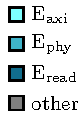
\includegraphics{assets/legend.pdf}
    }
    \hfill
    \subcaptionbox{PCM\label{fig:sunburst_avg_conf_proc_pcm}}{
        \import{assets/power_analysis}{pre}
\begin{tikzpicture}
    \pie[
        radius=2.3,
        text=pin,
        hide number,
    ]{
        1.2/1.2\%,
        2.6/2.6\%,
        5.0/5.0\%,
        3.0/3.0\%
    }
    \pie[
        radius=2.3,
        hide number,
        color={gray, bluehue2, bluehue4, bluehue6},
        before number=\printonlylargeenough{2},
        after number=\ifprintnumber\%\fi
    ]{
        1.2/,
        2.6/,
        5.0/,
        3.0/
    }
    \pie[
        radius=1.8,
        text=inside,
        color={blue!60, red!60},
    ]{
        11.8/$\econf$,
        88.2/$\eproc$
    }
\end{tikzpicture}

    }
    \caption{Average energy consumption distribution of the models listed in \cref{tab:example_models_stats}}
    \label{fig:example_models_avg_conf_proc}
\end{figure}

% When performing configuration and processing at \SI{60}{FPS}, we get the power values as shown in \cref{tab:example_models_power_consumption}.
Ideally, the energy consumption of the configuration of a model should be as minimal as possible.
In \cref{ch:7}, we explore techniques for increasing configuration efficiency.

% \begin{table}[hbtp]
%     \centering
%     \begin{threeparttable}
%         \begin{tabular}{@{}lrrr@{}}
%             \toprule
%                                        & \multicolumn{2}{l}{\textbf{Conf. power (mW)}} & \textbf{Proc. power (mW)} \\ \cmidrule(l){2-3} 
%             \textbf{Model}             & \textit{LPDDR5X}  & \textit{PCM}    & \\ \midrule
%             efficientnet               & 56.0              & 24.8            & 151.6 \\
%             mobnetv2                   & 37.0              & 16.4            & 95.9 \\
%             object\_tracker              & 42.8              & 18.9            & 98.3 \\
%             object\_detector             & 66.3              & 29.4            & 593.6 \\
%             resnet50                   & 102.6             & 45.4            & 380.2 \\
%             resnet101\tnote{1}         & 390.2             & 172.8           & 1081.7 \\
%             resnet101\_pruned\tnote{1} & 208.9             & 92.5            & 1179.4 \\ \bottomrule
%         \end{tabular}
%         \begin{tablenotes}
%             \item[1] Combination of all parts
%         \end{tablenotes}
%     \end{threeparttable}
%     \caption{Power consumption of configuration (of the same model) and processing of an input frame at \SI{60}{Hz}}
%     \label{tab:example_models_power_consumption}
% \end{table}
    